%%%%% Example from LaTeX tutorial: https://en.wikibooks.org/wiki/LaTeX/Floats,_Figures_and_Captions
\documentclass[a4paper,12pt]{article}

\usepackage[english]{babel}
\usepackage{graphicx}
\usepackage{varioref}
\usepackage{readlatex}

\begin{document}

\begin{figure}[!ht]
  \caption{A picture of a gull.jpg.}
  \centering
    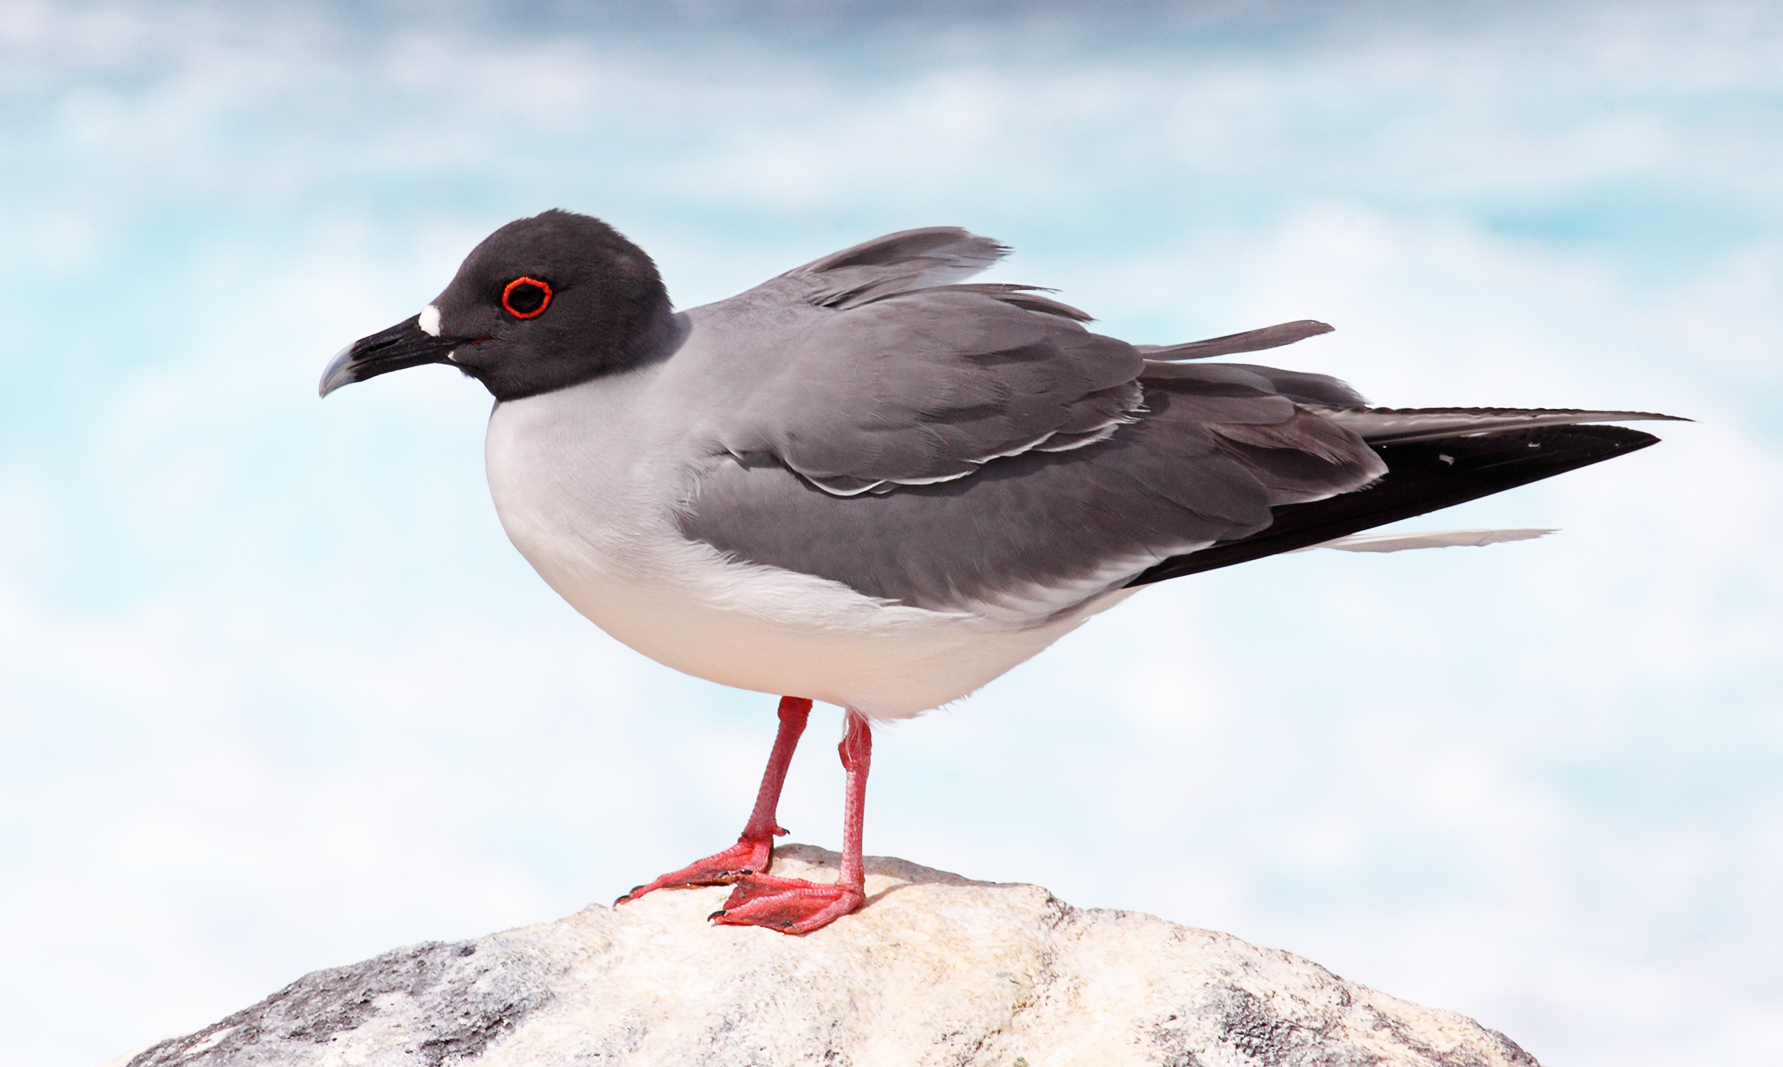
\includegraphics[width=0.5\textwidth]{gull.jpg}
\end{figure}

\begin{figure}[!ht]
  \centering
    \reflectbox{%
      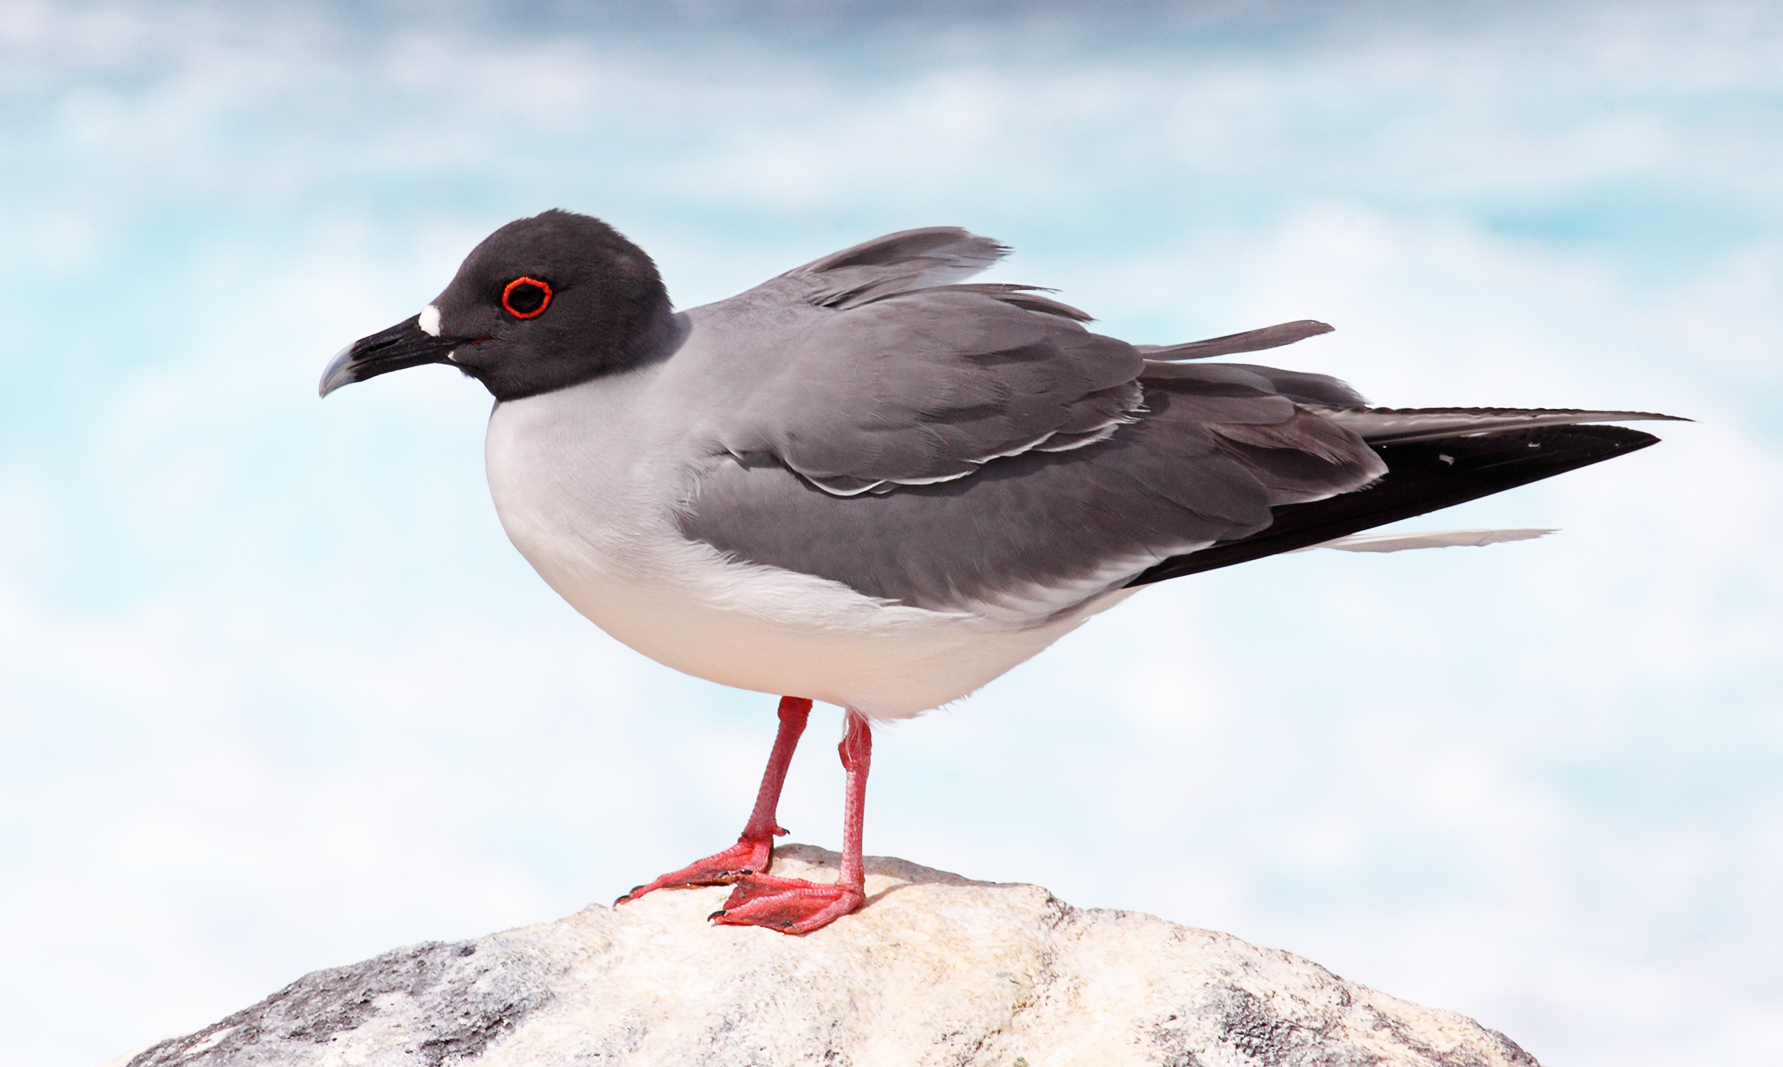
\includegraphics[width=0.5\textwidth]{gull.jpg}}
  \caption{A picture of the same gull.jpg
           looking the other way!}
\end{figure}

\begin{table}[!ht]
  \begin{center}
    \begin{tabular}{| l c r |}
    \hline
    1 & 2 & 3 \\
    4 & 5 & 6 \\
    7 & 8 & 9 \\
    \hline
    \end{tabular}
  \end{center}
  \caption{A simple table}
\end{table}

Notice how the tables and figures
have independent counters.

\end{document}